\fenicschapter{Discrete Optimization of Finite Element Matrix Evaluation}
              {Discrete Optimization of Finite Element Matrix Evaluation}
              {Robert C. Kirby, Matthew G. Knepley, Anders Logg, L. Ridgway Scott and Andy R. Terrel}
              {[kirby-4]}

\vspace{-0.5cm}

The tensor contraction structure for the computation of the element
tensor~$A^K$ obtained in Chapter~[logg-4] enables not only the
construction of a compiler for variational forms, but an
\emph{optimizing} compiler. For typical variational forms, the
reference tensor~$A^0$ has significant structure that allows the
element tensor~$A^K$ to be computed on an arbitrary element~$K$ in a
reduced amount of arithmetic. Reducing the number of operations based
on this structure leads naturally to several problems in discrete
mathematics.  This chapter introduces the kind of optimizations that
are possible and discusses compile-time combinatorial optimization
problems that form the core of the FErari
project.~\cite{KirbyLoggEtAl2006,KirbyScott2007,KirbyLogg2008,www:ferari}

We consider two basic kinds of optimizations in this chapter. First,
we consider relations between pairs of rows in the reference tensor.
This naturally leads to a graph that models proximity among these
pairs in the sense that if two rows are "close" together, then one may
reuse results computed with the first row to compute with the second.
This gives rise to a weighted graph that is (almost) a metric space,
so we designate such optimizations "topological". Second, we consider
relations between more than two rows of the reference tensor. Such
relations typically rely on sets of rows, considered as vectors in
Euclidean space, lying in a lower-dimensional space. Because we are
using planes and hyperplanes to reduce the amount of computation, we
describe these optimizations as "geometric".

\section{Optimization Framework}

The tensor paradigm developed in Chapter~[logg-4] arrives at the
representation
\begin{displaymath}
  A^K_i = \sum_{\alpha\in\mathcal{A}} A^0_{i\alpha} G_K^{\alpha},
  \quad i \in \mathcal{I},
\end{displaymath}
or simply
\begin{equation} \label{eq:kirby4:contract}
  A^K = A^0 : G_K,
\end{equation}
where $\mathcal{I}$ is the set of admissible multiindices for the
element tensor $A^K$ and $\mathcal{A}$ is the set of admissible
multiindices for the geometry tensor $G_K$. The reference tensor \(
A^0 \) can be computed at compile-time, and may then be contracted
with a \( G_K \) to obtain the element tensor $A^K$ for each cell \( K
\) in the finite element mesh at run-time.
The case of computing finite element stiffness matrices of size $n_K
\times n_K$, where $n_K$ is the dimension of the local finite element
space on $K$, corresponds to \( \mathcal{I} \) consisting of
$|\mathcal{I}| = n_K^2$ multiindices of length~two.

It is convenient to recast~(\ref{eq:kirby4:contract}) in terms of a
matrix--vector product:
\begin{equation} \label{eq:kirby4:tildeag}
  A^0 : G_K \leftrightarrow \tilde{A}^0 \tilde{g}_K.
\end{equation}
The matrix \( \tilde{A} \) lies in \( \mathbb{R}^{|\mathcal{I}| \times
  |\mathcal{A}|} \), and the vector \( \tilde{g}_{K} \) lies in
\( \mathbb{R}^{|\mathcal{A}|} \). The resulting matrix--vector product can
then be reshaped into the element tensor $A^K$. As this
computation must occur for each cell \( K \) in a finite element mesh,
it makes sense to try to make this operation efficient.

In the following, we will drop the subscripts and superscripts
of~(\ref{eq:kirby4:tildeag}) and consider the problem of computing
\[
y = A x
\]
efficiently, where \( A = \tilde{A}^0 \) is a fixed matrix
known \emph{a priori} and \( x = g_K \) is an arbitrary vector. We
will study structure of \( A \) that enables a reduction in the amount
of arithmetic required to form these products.

Before proceeding with the mathematical formulation, we give an
example of a matrix \( A \) that we would like to
optimize. In~(\ref{eq:kirby4:ALap}), we display the $6 \times 6 \times
2 \times 2$ reference tensor $A^0$ for computing a standard stiffness
matrix discretizing the Laplacian with quadratic Lagrange elements on
triangles. The rank four tensor is here depicted as a $6 \times 6$
matrix of $2 \times 2$ matrices. Full analysis would use a
corresponding flattened $36 \times 4$ matrix $A$.

% Laplacian with quadratic triangular Lagrange elements
\begin{equation} \label{eq:kirby4:ALap}
A^0 =
\left(
\begin{array}{cc|cc|cc|cc|cc|cc}
3 & 0 & 0 & -1 & 1 & 1 & -4 & -4 & 0 & 4 & 0 & 0 \\
0 & 0 & 0 & 0 & 0 & 0 & 0 & 0 & 0 & 0 & 0 & 0 \\ \hline
0 & 0 & 0 & 0 & 0 & 0 & 0 & 0 & 0 & 0 & 0 & 0 \\
-1 & 0 & 0 & 3 & 1 & 1 & 0 & 0 & 4 & 0 & -4 & -4 \\ \hline
1 & 0 & 0 & 1 & 3 & 3 & -4 & 0 & 0 & 0 & 0 & -4 \\
1 & 0 & 0 & 1 & 3 & 3 & -4 & 0 & 0 & 0 & 0 & -4 \\ \hline
-4 & 0 & 0 & 0 & -4 & -4 & 8 & 4 & 0 & -4 & 0 & 4 \\
-4 & 0 & 0 & 0 & 0 & 0 & 4 & 8 & -4 & -8 & 4 & 0 \\ \hline
0 & 0 & 0 & 4 & 0 & 0 & 0 & -4 & 8 & 4 & -8 & -4 \\
4 & 0 & 0 & 0 & 0 & 0 & -4 & -8 & 4 & 8 & -4 & 0 \\ \hline
0 & 0 & 0 & -4 & 0 & 0 & 0 & 4 & -8 & -4 & 8 & 4 \\
0 & 0 & 0 & -4 & -4 & -4 & 4 & 0 & -4 & 0 & 4 & 8 \\
\end{array}
\right)
\end{equation}

\section{Topological Optimization}

It is possible to apply the matrix $A$ depicted
in~(\ref{eq:kirby4:ALap}) to an arbitrary vector $x$ in fewer
operations than a standard matrix--vector multiplication which
requires $144$ multiply--add pairs. This requires offline analysis of
$A$ and special-purpose code generation that applies the particular
$A$ to a generic $x$. For \( A \in \mathbb{R}^{M\times N} \), let $\{
a^i \}_{i=1}^M \subset \mathbb{R}^N$ denote the rows of \( A \).  The
vector \( y = Ax \) may then be computed by \( M \) dot products of
the form \( y_i = a^i x \).  Below, we investigate relationships among
the rows of \( A \) to find an optimized computation of the
matrix--vector product.

For examination of $A$, we consider the following small subset
of~(\ref{eq:kirby4:ALap}) which would only cost $40$ multiply--add
pairs but contains all the relations we use to optimize the larger
version:

\begin{equation} \label{eq:kirby4:Aflat}
A =
\left(
\begin{array}{c}
  a^1 \leftrightarrow A^0_{1,3} \\
  a^2 \leftrightarrow A^0_{1,4} \\
  a^3 \leftrightarrow A^0_{2,3} \\
  a^4 \leftrightarrow A^0_{3,3} \\
  a^5 \leftrightarrow A^0_{4,6} \\
  a^6 \leftrightarrow A^0_{4,4} \\
  a^7 \leftrightarrow A^0_{4,5} \\
  a^8 \leftrightarrow A^0_{5,6} \\
  a^9 \leftrightarrow A^0_{6,1} \\
  a^{10} \leftrightarrow A^0_{6,6} \\
\end{array}
\right)
 =
\left(
\begin{array}{cccc}
1 & 1 & 0 & 0 \\
-4 & -4 & 0 & 0 \\
0 & 0 & 1 & 1 \\
3 & 3 & 3 & 3 \\
0 & 4 & 4 & 0 \\
8 & 4 & 4 & 8 \\
0 & -4 & -4 & -8 \\
-8 & -4 & -4 & 0 \\
 0 & 0 & 0 & 0 \\
8 & 4 & 4 & 8 \\
\end{array}
\right).
\end{equation}
%
A brief inspection of~(\ref{eq:kirby4:Aflat}) shows that \( a^9 \) is
zero; therefore, it does not need to be multiplied by the entries
of \( x \). In particular, if \( z \) entries of \( a^i \) are zero,
then the dot product \( a^i x \) requires \( N - z \) multiply--add
pairs rather than \( N \).

Suppose \( a^i = a^j \) for some \( i \neq j \), as seen in the sixth
and tenth rows of \( A \).  Then of course \( y_i = y_j
\), and only one dot product needs to be performed instead of two. In
other cases, \( \alpha a^i = a^j \) for some number \( \alpha \), as
in the first and second rows of~$A$. This means that after \( y_i \)
has been computed, then \( y_j = \alpha y_i \) may be computed with a
single multiplication.

In addition to equality and colinearity as above, one may also
consider other relations between the rows of $A$. A further inspection
of $A$ in~(\ref{eq:kirby4:Aflat}) reveals rows that have some entries
in common but are neither equal nor colinear. Such rows have a small
\emph{Hamming distance}, that is, the number of entries in which the
two rows differ is small. This occurs frequently, as seen in, e.g.,
rows five and six . Write \( a^j = a^i + (a^j-a^i) \). Then \( a^j -a^i
\) only has \( d \) nonzero entries, where $d$ is the Hamming distance
between $a^i$ and $a^j$.  Once \( y_i \) has been computed, one may
thus compute $y_j$ by
\[
y_j = y_i + \left( a^j - a^i \right) x,
\]
which requires only \( d \leq N \) additional multiply--add pairs. If
\( d \) is small compared to \( N \), the savings are considerable.

In a recent article~\cite{WolfHeath2009}, Heath and Wolf extend binary
relations to include the partial colinearity of two vectors.  For
example, the sixth and seventh rows have parts that are colinear,
namely \(a^6_{2:4} = - a^7_{2:4}\). Such relationships reduce the
computation of \(y_j\) to two multiply--add pairs; first a scaling of
the result computed with $y_j$ and then an additional multiplication
with the non-matching entry in $a^j$.

All of these examples of structure either relate to a single row of \(
A \) or else to a pair of rows of \( A \). Such \emph{binary}
relations between pairs of rows are amenable to the formulation of
graph-theoretic structures, as is developed in
Section~\ref{sec:kirby4:graph}. Higher-order relations also occur
between the rows of \( A \).  For example, the first and third rows
may be added and scaled to make the fourth row.  In this case, once \(
a^1 x \) and \( a^2 x \) are known, the results may be used to
compute \( a^{4} x \) using one addition and one multiplication,
compared to four multiplications and three additions for direct
evaluation of the dot product $a^{4} x$.

\section{A Graph Problem}
\label{sec:kirby4:graph}

If we restrict consideration to binary relations between the rows of
\( A \), we are led naturally to a weighted, undirected graph whose
vertices are the rows \( a^i \) of $A$.  An edge between \( a^i \) and
\( a^j \) with weight \( d \) indicates that if \( a^i x \) is known
for some \( x \), then that result may be used to compute \( a^j x \)
with \( d \) multiply--add pairs.  In practice, such edges also need to
be labeled with information indicating the kind of relationship such
as equality, colinearity or low Hamming distance.

To find the optimal computation through the graph, we use Prim's
algorithm~\cite{prim} for computing a minimum-spanning tree. A minimum
spanning tree is a tree that connects all the vertices of the graph
and has minimum total edge weight. In~\cite{KirEtAl2006}, it is
demonstrated that, under a given set of relationships between rows, a
minimum spanning tree in fact encodes an algorithm that optimally
reduces arithmetic.  This discussion assumes that the initial graph is
connected. In principle, every \( a^i \) is no more than a distance
of \( N \) away from any \( a^j \). In practice, however, only
edges \( N - z \) are included in a graph since $N$ is the cost of
computing \( y_i \) without reference to \( y_j \). This often makes
the graph unconnected and thus one must construct a minimum
spanning \emph{forest} instead of a tree (a set of disjoint trees that
together touch all the vertices of the graph). An example of a minimum
spanning tree using the binary relations is shown in
Figure~\ref{fig:kirby4:mst}.

\begin{figure}
  \begin{center}
   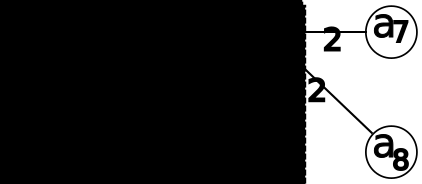
\includegraphics[width=\smallfig]{chapters/kirby-4/pdf/small_mst.pdf}
    \caption{Minimum spanning tree (forest) for the vectors in
      (\ref{eq:kirby4:Aflat}). The dashed edges represent edges that do
    not reduce the number of operations and thus disconnect the graph.}
    \label{fig:kirby4:mst}
  \end{center}
\end{figure}

Such a forest may then be used to determine an efficient algorithm for
evaluating \( A x \) as follows. Start with some \( a^i \) and
compute \( y^i = a^i x \) directly in at most \( N \) multiply--add
pairs. The number of multiply--add pairs may be less than one if one
or more entries of $a^i$ are zero. Then, if \( a^j \) is a nearest
neighbor of \( a^i \) in the forest, use the relationship between \(
a^j \) and \( a^i \) to compute \( y^j = a^j x \).  After this, take a
nearest neighbor of \( a^j \), and continue until all the entries of
\( y \) have been computed.

Additional improvements may be obtained by recognizing that the input
tensor \( G_K \leftrightarrow x \) is symmetric for certain operators
like the Laplacian. In two space dimensions, \( G_K \) for the
Laplacian is \( 2 \times 2 \) with only 3 unique entries, and in three
space dimensions it is \( 3 \times 3 \) with only 6 unique entries.
This fact may be used to construct a modified reference tensor \(
A^0 \) with fewer columns.  For other operators, it might have
symmetry along some but not all of the axes.

Heath and Wolf proposed a slight variation on this algorithm.  Rather
than picking an arbitrary starting row \( a^i \), they enrich the
graph with an extra vertex labeled \textit{IP} for ``inner product.''
Each \( a^i \) is a distance \( N - z \) from IP, where \( z \) is the
number of vanishing entries in \( a^i \).  The IP vertex is always
selected as the root of the minimum spanning tree.  It allows for a
more robust treatment of unary relations such as sparsity, and
detection of partial colinearity relations.

\section{Geometric Optimization}
\label{sec:kirby4:geom}

When relations between more than two rows are considered, the
optimization problem no longer may be phrased in terms of a graph, but
requires some other structure.  In these cases, proving that one has
found an optimal solution is typically difficult, and it is suspected
that the associated combinatorial problems are \( NP \)-hard.

As a first attempt, one can work purely from linear dependencies among
the data as follows.  Let \( B=\{ b^i \}_i \subseteq \{ a^i \}_{i=1}^N
\) be a maximal set of nonzero rows of \( A \) such that no two rows
are colinear. Then enumerate all triples which are linearly dependent,
\begin{displaymath}
  T = \left\{ \left\{ b^i , b^j , b^k \right\} \subseteq B:
  \exists \, \alpha_1, \alpha_2, \alpha_3 \neq 0:
  \alpha_1 b^i + \alpha_2 b^j + \alpha_3 b^k = 0 \right\}.
\end{displaymath}
The idea is now to identify some subset $C$ of \( B \) that may be
used to recursively construct the rest of the rows in \( B \) using
the relationships in \( T \).

Given some \( C \subset B \), we may define the \emph{closure} of \(
C \), denoted by \( \bar{C} \), as follows.  First of all, if \( b
\in C \), then \( b \in \bar{C} \).  Second, if \( b \in B \) and
there exist \( c,d \in \bar{C} \) such that \( \{b,c,d\} \in T \),
then \( b \in \bar{C} \) as well.  If \( \bar{C} = B\), we say
that \( C \) is a \emph{generator} for \( B \) or that \( C \)
\emph{generates} \( B \).

The recursive definition suggests a process for constructing the
closure of any set \( C \).  In the course of constructing the
closure, one may also construct a directed, acyclic graph that
indicates the linear dependence being used.  Each \( b \in C \) will
have no out-neighbors, while each \( b \in \bar{C} \backslash C \)
will point to two other members of \( \bar{C} \).  This graph is
called a \emph{generating graph}. Using (\ref{eq:kirby4:Aflat}), we
have the following sets $B$, $T$, and $C$, with the generating graph
shown in Figure~\ref{fig:kirby4:gg}:
\begin{displaymath}
\begin{array}{rcl}
 B & = &  \{a_1, a_3, a_4, a_5, a_6, a_7, a_8\} \\
 T & = & \{(a_1, a_3, a_4),(a_4, a_5, a_6), (a_6, a_7, a_8)\} \\
 C & = & \{a_3, a_4, a_5, a_7\} \\
\end{array}
\end{displaymath}

\begin{figure}
  \begin{center}
 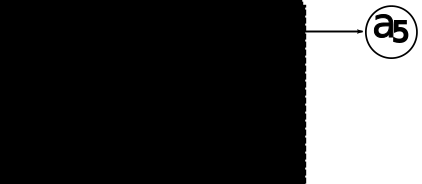
\includegraphics[width=\smallfig]{chapters/kirby-4/pdf/gg2.pdf}
  \caption{Generating graph for the vectors in~(\ref{eq:kirby4:Aflat}).}
  \label{fig:kirby4:gg}
  \end{center}
\end{figure}

If $C$ generates \( B \), then the generating graph indicates an
optimized (but perhaps not optimal) process for computing \( \{ y^i =
b^i x \}_i\).  Take a topological ordering of the vectors \( b^i \)
according to this graph.  Then, for each \( b^i \) in the topological
ordering, if \( b^i \) has no out neighbors, then \( b^i x \) is
computed explicitly.  Otherwise, \( b^i \) will point to two other
vectors \( b^j \) and \( b^k \) for which the dot products with \( x
\) will already be known. Since the generating graph has been built
from the set of linearly dependent triples~$T$, there must exist some
\( \beta_1, \beta_2 \) such that \( b^i = \beta_1 b^j + \beta_2 b^k
\). We may thus compute $y^i$ by
\[
y^i = b^i x = \beta_1 b^j x
+ \beta_2  b^k  x,
\]
which requires only two multiply--add pairs instead of \( N \).

To make best use of the linear dependence information, one would like
to find a generator \( C \) that has as few members as possible.  We
say that a generator \( C \) is \emph{minimal} for $B$ if no \( C'
\subset C \) also generates \( B \). A stronger requirement is for a
generator to be \emph{minimum}. A generator $C$ is minimum if no other
generator $C'$ has lower cardinality. Heuristics for constructing
minimal generators are considered in~\cite{KirSco2007}, and it is not
currently known whether such heuristics construct minimum generators
or how hard the problem of finding minimum generators is.

Given a minimal generator \( C \) for \( B \), one may consider
searching for higher order linear relations among the elements of \(
C \), such as sets of four items that have a three-dimensional span.
The discussion of generating graphs and their utilization is the same
in this case.

Wolf and Heath~\cite{WolfHeath2009} study combining binary and
higher-order relations between the rows of \( A \) in a hypergraph
model.  While greedy algorithms provide optimal solutions for a graph
model, they demonstrate that the obvious generalizations to
hypergraphs can be suboptimal.  While the hypergraph problems are most
likely very hard, they develop heuristics that perform well and
provide additional optimizations beyond the graph models.  So, even if
a non-optimal solution is found, it still provides improved reduction
in arithmetic requirements.

\begin{table}
  \begin{center}
    \begin{tabular}{c|c}
      triangles & tetrahedra \\
      \begin{tabular}{c|ccc|c}\hline
        degree & $M$ & $N$ & $MN$ & MAPs \\
        \hline
        1 &6 &3& 18& 9 \\
        2 &21& 3& 63& 17\\
        3 &55& 3& 165& 46 \\\hline
      \end{tabular}
      &
      \begin{tabular}{c|ccc|c}\hline
        degree & $M$ & $N$ & $MN$ & MAPs \\
        \hline
        1 & 10 & 6 &60 &27 \\
        2 & 55 & 6 & 330 &101 \\
        3 & 210 &6 &1260 &370 \\\hline
      \end{tabular}
    \end{tabular}
    \label{tab:kirby4:graph}
    \caption{Number of multiply--add pairs for graph-optimized Laplace
      operator (MAPS) compared to the basic number of multiply--add pairs ($MN$).}
  \end{center}
\end{table}

In Table~\ref{tab:kirby4:geom}, topological and geometric optimization
is compared for the Laplacian using quadratic through quartic
polynomials on tetrahedra.  In the geometric case, the vectors \( a^i
\) were filtered for unique direction, i.e., only one vector for each
class of colinear vectors was retained. Then, a generating graph was
constructed for the remaining vectors using pairwise linear
dependence.  The generator for this set was then searched for linear
dependence among sets of four vectors, and a generating graph
constructed.  Perhaps surprisingly, the geometric optimization found
flop reductions competitive with or better than graph-based binary
relations. These are shown in Table~\ref{tab:kirby4:geom}.

\begin{table}
  \begin{center}
    \begin{tabular}{c|ccc}
      & 2 & 3 & 4 \\ \hline
      topological & 101 & 370 & 1118 \\
      geometric   & 105 & 327 & 1072 \\
    \end{tabular}
    \caption{Comparison of topological and geometric optimizations
      for the Laplace operator on tetrahedra using polynomial degrees two
      through four. In each case, the final number of MAPs for the
      optimized algorithm is reported. The case $q=1$ is not reported
      since then both strategies yield the same number of operations.}
  \end{center}
  \label{tab:kirby4:geom}
\end{table}

\section{Optimization by Dense Linear Algebra}

As an alternative to optimizations that try to find a reduced
arithmetic for computing the element tensor~$A^K$, one may consider
computing the element tensor by efficient dense linear algebra.  As
above, we note that the entries of the element tensor $A^K$ may be
computed by the matrix--vector product $\tilde{A}^0
\tilde{g}_K$. Although zeros may appear in $\tilde{A}^0$, this is
typically a dense matrix and so the matrix--vector product may be
computed efficiently with Level~2 BLAS, in particular using a call
to~\texttt{dgemv}. There exist a number of optimized implementations
of BLAS, including hand-optimized vendor implementations, empirically
and automatically tuned libraries~\cite{blas} and formal methods for
automatic derivation of algorithms~\cite{flame}.

The computation of the element tensor $A^K$ may be optimized further
by recognizing that one may compute the element tensor for a batch of
elements $\{K_i\}_i \subset \mathcal{T}$ in one matrix--matrix
multiplication:
\begin{displaymath}
  \left[\tilde{A}^0 \tilde{g}_{K_1} \quad \tilde{A}^0 \tilde{g}_{K_2} \quad \cdots \right] =
  \tilde{A}^0 \left[\tilde{g}_{K_1} \quad \tilde{g}_{K_2} \quad \cdots\right].
\end{displaymath}
This matrix-matrix product may be computed efficiently using a single
Level~3 BLAS call (\texttt{dgemm}) instead of a sequence of Level~2
BLAS calls, which typically leads to better floating-point
performance.

\section{Notes on Implementation}

A subset of the optimizations discussed in this chapter are available
as part of the FErari Python module. The current version of FErari
(0.2.0) implements optimization based on finding binary relations
between the entries of the element tensor. With optimizations turned
on, FFC calls FErari at compile-time to generate optimized
code. Optimization for FFC can be turned on either by the \texttt{-O}
parameter when FFC is called from Python, or by setting
\begin{verbatim}
  parameters["form_compiler"]["optimization"] = True
\end{verbatim}
when FFC is called as a just-in-time compiler from the DOLFIN Python
interface. Note that the FErari optimizations are only used when FFC
generates code based on the tensor representation described in
Chapter~[logg-4]. When FFC generates code based on quadrature,
optimization is handled differently, as described in
Chapter~[oelgaard-2].
